
\chapter{枝刈りによる探索空間の削減}
\label{chap:reduce-by-prune}
枝刈りによって探索空間を削減する.
本稿では,直径の下界を計算し,定理\ref{thm:gmg-geometric-property}
の条件\ref{gmg-geom-b}を満足するか求めることで実現する.

\section{直径の下界の計算}
\label{sect:distance-lower-bound}
直径の下界を計算する方法を与える.まず,次のグラフを定義する.
\begin{definition}
  探索途中のグラフ$G$が与えられ,$i$番目の辺$e_i\in E$の追加判定および追加が
  行われたとする.$G$の辺と追加が未決定の辺すべて($\{e_j\}_{j>i}\subseteq E$)
  を合わせたグラフを\textbf{最大グラフ}と定義する.
  このとき,最大グラフのもとになったグラフを\textbf{最小グラフ}と呼ぶ.
\end{definition}
\begin{example}
  図\ref{fig:min-max-graph}に例を示す.最小グラフの破線部分は追加の
  判定が行われていない辺を表す.最大グラフは,最小グラフの追加未決定の辺を
  すべて追加したグラフとなっている.
\end{example}
\begin{figure}
  \centering
  \subfloat[最小グラフ]{
    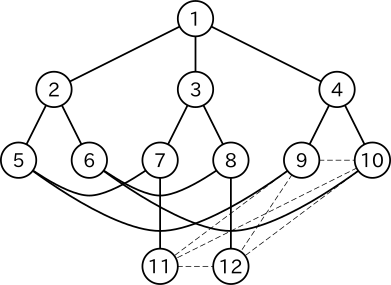
\includegraphics[width=.4\linewidth]
                    {min-graph-example.pdf}
  }\hfill
  \subfloat[最大グラフ]{
    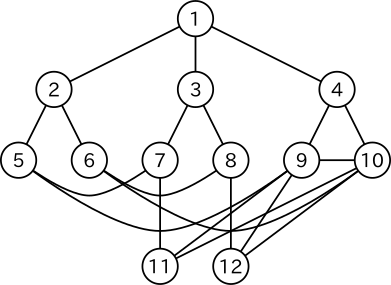
\includegraphics[width=.4\linewidth]
                    {max-graph-example.pdf}
  }
  \caption{最小グラフと最大グラフの例}
  \label{fig:min-max-graph}
\end{figure}

直径の下界は,最大グラフの直径を計算すればよい.もし直径の下界が
定理\ref{thm:gmg-geometric-property}の条件\ref{gmg-geom-b}を
満たさない場合,それはどのように辺を追加しても条件を満たさないので,
その場で探索を打ちきることができる.

\section{頂点間距離の高速な更新法}
\label{sect:faster-min-max}
第\ref{chap:basic-algorithm}章にて,グラフが枝刈りの対象となるかを
判定するには,追加する辺の頂点間距離と直径の下界を求める必要があることを述べた.
本節では,これらの値を高速に計算するため,辺の追加と削除に対して,頂点間距離と
直径の下界を更新するアルゴリズムを与える.
探索空間の削減にはつながらないが,計算量が削減され,実行時間の短縮が期待できる.
また,この方法は辺の追加と削除に対する媒介中心性の高速な計算法への応用が期待できる.

グラフ$G=(V,E),V=\{1,\ldots n\}$のすべての頂点の組$(s,t)$の距離$d(s,t)$と
距離が$d(s,t)$となる最短経路の数$\sigma(s,t)$が与えられているとする.
まず,追加と削除に共通するいくつかの補題を示す.
\begin{lemma-without-proof}[Brandes\cite{Brandes2001}]
  $G=(V,E)$の異なる2頂点$s,t\in V$に対して,$s$から$t$への最短経路
  $G_{st}=(V_{st},E{st})$が$i\in V$を含む,すなわち$i\in V_{st}$であるための
  必要十分条件は
  \[ d(s,t)=d(s,i)+d(i,t) \]
  が成り立つことである.
\end{lemma-without-proof}
\begin{lemma-without-proof}[難波ら\cite{Namba2016}]
  $G=(V,E)$の異なる2頂点$s,v\in V$と辺$\{i,j\}\in E$を考える.
  $s$から$t$への最短経路$G_{st}=(V_{st},E_{st})$が有向辺$(i,j)$を含む,
  すなわち$(i,j)\in E_{st}$が成り立つための必要十分条件は
  \[ d(s,t)=d(s,i)+d(j,t)+1 \]
  が成り立つことである.
\end{lemma-without-proof}
\begin{lemma-without-proof}[Brandes\cite{Brandes2001}]
  $G=(V,E)$の異なる2頂点$s,t\in V$に対して,$s$から$t$への最短経路の中で
  $i$を通るものの個数$\sigma_{st}(i)$は次式で与えられる.
  \[ \sigma(s,t)=\begin{aligned}\begin{cases}
    \sigma(s,i)\sigma(i,t) & d(s,t)=d(s,i)+d(i,t)\mathrm{のとき} \\
    0 & \mathrm{それ以外のとき}
  \end{cases}\end{aligned} \]
\end{lemma-without-proof}

次の補題は,ある2頂点間の最短経路の個数と,その経路に含まれる
短い最短経路の個数との関係を示す.
\begin{lemma}
  \label{lemma:number-of-paths}
  $d(s,t)=d(s,v)+d(v,t)$である$v\in V$(ただし$v\neq s,v\neq t$)について,
  \begin{equation}
    \label{eq:number-of-paths}
    \sigma(s,t)=\left(
    \sum_{v}\sigma(s,v)\sigma(v,t)\right) / (d(s,t)-1)
  \end{equation}
  が成り立つ.
\end{lemma}
\begin{proof}
  $s$と$t$の間の一般的な経路を図\ref{fig:proof-number-of-paths}に示す.
  \begin{figure}
    \centering
    \def\svgwidth{.5\columnwidth}
    \input{proof-number-of-paths.pdf_tex}
    \caption{$s$と$t$の一般的な最短経路}
    \label{fig:proof-number-of-paths}
  \end{figure}
  $s$からの距離が一定の頂点を並べて,一つの層とする.$d(s,v)=k$なる頂点
  $v$の集合を,第$k$層と定義し,$L_k$と表す.
  $L_k$に属する頂点の数を$n_k$,$l$番目の頂点を$v_{kl}$と表す.
  ここで,すべての層に属する頂点$v$は,隣接する層以外の層に属する頂点$w$と
  隣接しないことに注意する.もしそのような頂点が存在すると,最短経路長が
  変化する.式\ref{eq:number-of-paths}の両辺に$d(s,t)-1$を掛けて,
  \begin{equation}
    \sigma(s,t)(d(s,t)-1)=\sum_{v}\sigma(s,v)\sigma(v,t)
    \label{eq:number-of-paths1}
  \end{equation}
  となる.式\ref{eq:number-of-paths1}の右辺を,
  図\ref{fig:proof-number-of-paths}にならって変形して,
  \begin{equation}
    \sum_{v}\sigma(s,v)\sigma(v,t)=
    \sum_{k=1}^m\sum_{l=1}^{n_k}\sigma(s,v_{kl})\sigma(v_{kl},t)
    \label{eq:number-of-paths2}
  \end{equation}
  とする.二つの頂点$v$と$w$について,
  \begin{align*}
    a(v,w)=
    \begin{cases}
      1 & vとwが隣接しているとき \\
      0 & vとwが隣接していないとき
    \end{cases}
  \end{align*}
  と定義する.
  各々の$\sigma(s,v_{kl})\sigma(v_{kl},t)$について議論する.
  定義に沿って式を変形すると,
  \begin{align}
    &\sigma(s,v_{kl})\sigma(v_{kl},t)\nonumber\\
    =&\left(\sum_{v'\in L_{k-1}}\sigma(s,v')a(v',v_{kl})\right)
    \left(\sum_{v'\in L_{k+1}}\sigma(v_{kl},v')a(v',t)\right)
    \nonumber\\
    =&\left(\sum_{v''\in L_{k-2}}\sum_{v'\in L_{k-1}}
    \sigma(s,v'')a(v'',v')a(v',v_{kl})\right)
    \left(\sum_{v'\in L_{k+1}}\sum_{v''\in L_{k+2}}
    a(v_{kl},v')a(v',v'')\sigma(v'',t)\right)
    \nonumber\\
    &\vdots\nonumber\\
    =&\left(\sum_{(v_1,\ldots,v_{k-1})\in L_1\times\cdots\times L_{k-1}}
    a(s,v_1)\cdots a(v_{k-1},v_{kl})\right)
    \left(\sum_{(v_{k+1},\ldots,v_m)\in L_{k+1}\times\cdots\times L_m}
    a(v_{kl},v_{k+1})\cdots a(v_m,v_t)\right)\nonumber\\
    =&\sum_{
      (v_1,\ldots,v_{k-1},v_{k+1},\ldots,v_m)\in
      L_1\times\cdots\times L_{k-1}\times L_{k+1}\times\cdots\times L_m
    }
    a(s,v_1)\cdots a(v_{k-1},v_{kl})a(v_{kl},v_{k+1})\cdots a(v_m,t)
    \label{eq:number-of-paths3}
  \end{align}
  となる.式\ref{eq:number-of-paths3}を式\ref{eq:number-of-paths2}に
  代入すると,
  \begin{align}
    &\sum_{k=1}^m\sum_{l=1}^{n_k}\sigma(s,v_{kl})\sigma(v_{kl},t)\nonumber\\
    =&\sum_{k=1}^m\sum_{l=1}^{n_k}\sum_{
      (v_1,\ldots,v_{k-1},v_{k+1},\ldots,v_m)\in
      L_1\times\cdots\times L_{k-1}\times L_{k+1}\times\cdots\times L_m
    }
    a(s,v_1)\cdots a(v_{k-1},v_{kl})a(v_{kl},v_{k+1})\cdots a(v_m,t)\nonumber\\
    =&\sum_{k=1}^m\sum_{(v_1,\ldots,v_m)\in L_1\times\cdots\times L_m}
    a(s,v_1)\cdots a(v_m,t)\nonumber\\
    =&m\left(\sum_{(v_1,\ldots,v_m)\in L_1\times\cdots\times L_m}
    a(s,v_1)\cdots a(v_m,t)\right)
    \label{eq:number-of-paths4}
  \end{align}
  とできる.式\ref{eq:number-of-paths4}の総和の対象が$1$となるのは,
  $a(s,v_1),\ldots,a(v_m,t)$のすべてが$1$のとき,
  すなわち,$s$と$t$の最短経路となっているときである.
  従って,総和の値は$s$と$t$の最短経路の数を一致し,
  式\ref{eq:number-of-paths4}は$m\sigma(s,t)$と等しい.
\end{proof}

\subsection{辺の追加に対する頂点間距離の更新}
\label{subsect:update-path-length}
$G$に辺$e=\{\alpha,\beta\}\notin E(G)$を追加したた後の頂点間距離$d'(s,t)$と
最短経路数$\sigma'(s,t)$を求める.
一般性を失うことなく,$s<t,\,d(s,\alpha)\leq d(s,\beta)$とできる.

アルゴリズムをアルゴリズム\ref{algo:update-distance-on-insert}に示す.
\begin{algorithm}
  \caption{辺$\{\alpha,\beta\}$が追加されたときの$d'(s,t)$と$\sigma'(s,t)$の
  計算}\label{algo:update-distance-on-insert}
  \begin{algorithmic}[1]
    \Require $G=(V,E),\,d(s,t),\,\sigma(s,t)$
    \Ensure $d'(s,t),\,\sigma'(s,t)$
    \State $d'$と$\sigma'$の初期値を$d$と$\sigma$の値にしておく
    \ForAll{$(s,t)\in V\times V,\,s<t$}
    \State $(\alpha,\beta)$のうち$s$に近いほうを$\alpha$とする
    \If{$d(s,\alpha)<d(s,\beta)$かつ$d(s,t)>d(s,\alpha)+d(\beta,t)+1$}
    \State $d'(s,t)\gets d(s,\alpha)+d(\beta,t)+1$
    \State $d'(t,s)\gets d(s,\alpha)+d(\beta,t)+1$
    \State $\sigma'(s,t)\gets \sigma(s,\alpha)\sigma(\beta,t)$
    \State $\sigma'(t,s)\gets \sigma(s,\alpha)\sigma(\beta,t)$
    \ElsIf{$d(s,\alpha)<d(s,\beta)$かつ$d(s,t)=d(s,\alpha)+d(\beta,t)+1$}
    \State $\sigma'(s,t)\gets \sigma(s,t)+\sigma(s,\alpha)\sigma(\beta,t)$
    \State $\sigma'(t,s)\gets \sigma(s,t)+\sigma(s,\alpha)\sigma(\beta,t)$
    \Else
    \EndIf
    \EndFor
  \end{algorithmic}
\end{algorithm}

\subsection{辺の削除に対する頂点間距離の更新}
\label{subsect:update-lower-bound-of-diameter}
$G$から辺$e=\{\alpha,\beta\}\in E(G)$を削除した後の頂点間距離$d'(s,t)$と
最短経路数$\sigma'(s,t)$を求める.
一般性を失うことなく,$s<t,\,d(s,\alpha)\leq d(s,\beta)$とできる.

削除による影響を受けない場合は,$\cdots$である.
削除により,頂点間距離が変化せず,経路の個数が変化する場合は,$\cdots$である.
削除により,頂点間距離が変化する場合は,$\cdots$である.

次に,頂点間距離の更新が行われる組$(s,t)$の$\sigma'(s,t)$について議論する.
まず,準備のため次を示す.
\begin{collary}
  $\sigma'(s,t)$を再計算するには,すべての$d'(s,t)>d'(u,v)$の$\sigma'(u,v)$
  を先に計算しなければならない.
\end{collary}
\begin{proof}
  補題\ref{lemma:number-of-paths}の式\ref{eq:number-of-paths2}を見ると,
  $s$と$t$の最短経路の中に$d'(s,t)>d'(u,v)$なる$u$と$v$の最短経路が含まれ,
  そのような$u,v$に対する$\sigma'(u,v)$が含まれる.
\end{proof}
更新の対象となる頂点組の列$\{(s_i,t_i)\}$を更新後の距離$d'$の昇順に,
定理\ref{lemma:number-of-paths}の式を用いて,$\sigma'(u,v)$を求める.

アルゴリズムをアルゴリズム\ref{algo:update-distance-on-remove}に示す.
\begin{algorithm}
  \caption{辺$\{\alpha,\beta\}$が削除されたときの$d'(s,t)$と$\sigma'(s,t)$の
  計算}\label{algo:update-distance-on-remove}
  \begin{algorithmic}[1]
    \Require $G=(V,E),\,d(s,t),\,\sigma(s,t)$
    \Ensure $d'(s,t),\,\sigma'(s,t)$
    \State $d'$と$\sigma'$の初期値を$d$と$\sigma$の値にしておく
    \State $P\gets\varnothing$
    \Comment{更新の対象となる頂点組$(s,t)$}
    \ForAll{$(s,t)\in V\times V,\,s<t$}
    \State $\textrm{npath}\gets$\Call{Path num not contain}{$s,t$}
    \If{$d(s,t)=\infty$または$\textrm{npath}>0$}
    \State $\sigma'(s,t)\gets\textrm{npath},\:\sigma'(t,s)\gets\textrm{npath}$
    \Else\Comment{削除により頂点間距離が変化する}
    \State $d_{\min}\gets \infty$
    \ForAll{$v\in V$}
    \If{\Call{Path num not contain}{$s,v$}$>0$かつ
      \Call{Path num not contain}{$v,t$}$>0$}
    \State $d_{\min}\gets\min\left(d_{\min},d(s,v)+d(v,t)\right)$
    \EndIf
    \EndFor
    \If{$d_{\min}=\infty$}
    \Comment{削除により連結でなくなった}
    \State $d'(s,t)\gets\infty,\:d'(t,s)\gets\infty$
    \State $\sigma'(s,t)\gets 0,\:\sigma'(t,s)\gets 0$
    \Else
    \State $d'(s,t)\gets d_{\min},\:d'(t,s)\gets d_{\min}$
    \State \parbox[t]{\linewidth}{
      $P\gets \{\ldots,(s_i,t_i),(s,t),(s_{i+1},t_{i+1}),\ldots\}$\\
      ただし,$d'(s_i,t_i)\leq d'(s,t)\leq d'(s_{i+1},t_{i+1}),\:$
      $(s_1,t_1),\ldots,(s_i,t_i),\ldots\in P$
    }
    \EndIf
    \EndIf
    \EndFor
    \ForAll{$i=\{1,\ldots,|P|\}$}\Comment{最短経路数を更新}
    \State $(s_i,t_i)\gets P_i$
    \State \parbox[t]{\linewidth}{
      $\sigma'(s_i,t_i)\gets$
      $\left(\sum_{v}\sigma(s_i,v)\sigma(v,t_i)\right) / (d'(s_i,t_i)-1)$ \\
      ただし,
      $v\in V,\,d'(s_i,t_i)=d'(s_i,v_i)+d'(v_i,t_i),\,v\neq s_i,\,v\neq t_i$
    }
    \EndFor
    \Procedure{Path num not contain}{$s,t$}
    \State $(\alpha,\beta)$のうち$s$に近いほうを$\alpha$とする
    \If{$d(s,t)<d(s,\alpha)+d(\beta,t)+1$}
    \State \textbf{return} $\sigma(s,t)$
    \Else
    \State \textbf{return} $\sigma(s,t)-\sigma(s,\alpha)\sigma(\beta,t)$
    \EndIf
    \EndProcedure
  \end{algorithmic}
\end{algorithm}

\section{実験}

\section{結果}
次数が3のときの実験結果を示す.
探索開始から最初の一般化ムーアグラフの発見における探索時間と状態の
取り出し回数を図\ref{fig:sinitr-time}と図\ref{fig:sinitr-node}に
それぞれ示す.また,一般化ムーアグラフの列挙におけるグラフ数と列挙時間と
状態の取り出し回数を図\ref{fig:sinitr-full-graph}と図\ref{fig:sinitr-full-time}と
図\ref{fig:sinitr-full-node}にそれぞれ示す.結果から,次のことが考察される.
指数関数的に増える(適当).

\begin{figure}
  \centering
  \includegraphics{the-sinitr-time.pdf}
  \caption{最初の一般化ムーアグラフの発見までの時間}
  \label{fig:sinitr-time}
\end{figure}
\begin{figure}
  \centering
  \includegraphics{the-sinitr-node.pdf}
  \caption{最初の一般化ムーアグラフの発見までの展開状態数}
  \label{fig:sinitr-node}
\end{figure}

\begin{figure}
  \centering
  \includegraphics{the-sinitr-full-graph.pdf}
  \caption{列挙された一般化ムーアグラフの数}
  \label{fig:sinitr-full-graph}
\end{figure}
\begin{figure}
  \centering
  \includegraphics{the-sinitr-full-time.pdf}
  \caption{一般化ムーアグラフの列挙に要した時間}
  \label{fig:sinitr-full-time}
\end{figure}
\begin{figure}
  \centering
  \includegraphics{the-sinitr-full-node.pdf}
  \caption{一般化ムーアグラフの列挙における展開状態数}
  \label{fig:sinitr-full-node}
\end{figure}
